\begin{frame}[fragile]{Tracking: Git Objects}
  \begin{columns}
    \begin{column}{0.3\textwidth}
      Tree Objects
      \begin{flushleft}
        \footnotesize
contain one or more entries, each of which is the SHA-1 hash of a blob or
subtree with its mode, type, and filename. 
      \end{flushleft}
      Commit Objects
      \begin{flushleft}
        \footnotesize
contain the parent commits (if any), the top-level tree, the author/committer
information, and the commit message.
      \end{flushleft}
    \end{column}
    \begin{column}{0.7\textwidth}
      \begin{figure}
        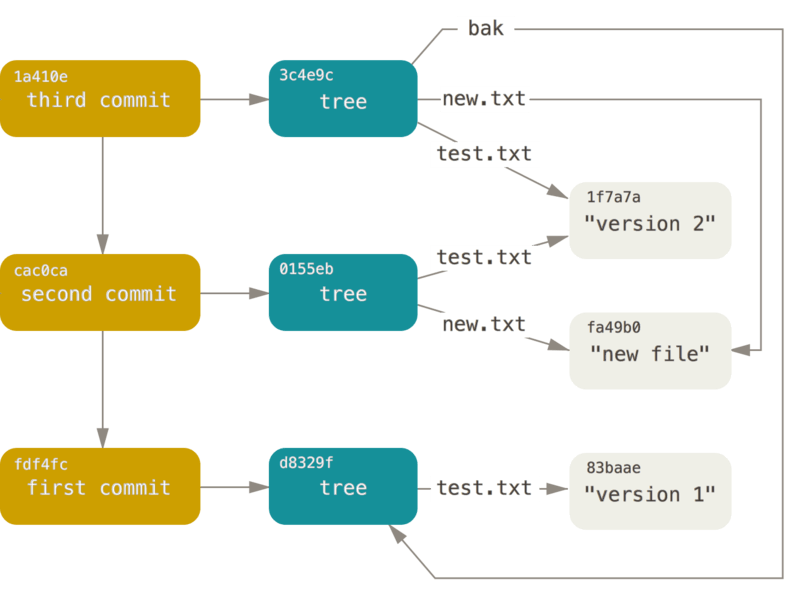
\includegraphics[width=\textwidth]{tracking/data-model-3}
        \caption{All the reachable objects in your Git directory}
      \end{figure}
      \begin{flushleft}
        \footnotesize
        The Git objects form a Directed Acyclic Graph (DAG).
      \end{flushleft}
    \end{column}
  \end{columns}
\end{frame}
